\chapter{Recommendations and Future Work}

In this dissertation, we have documented our work Co-designing an unemployment intervention for graduates of NGO-run job-readiness courses. We conclude with some recommendations for next steps and design parameters for this or similar contexts.

%------------------------------------------------
\section{Social-media Based Referral Systems}

In our findings, similar to a related research in India \cite{white2012}, we found that the job seekers make use of social communication networks such as Facebook and WhatsApp (even though they lack job searching skills) and as such it would be useful to implement a referral system where job seekers can be recommended by their previous Pease-jobs employers to assist them in finding other jobs. Integrated into the application prototyped in this research, the referrals and referees can then be mentioned in the cover letter generated for the job seekers to make for a reliable cover letter.

%------------------------------------------------
\section{Security of Personal Information}

For a system that collects personal information such as phone numbers, email addresses, and physical addresses, users should be aware that they would be giving out information and their information should be kept secure. A thorough ‘terms and conditions’ section should be available stating what can be done with participant information in the case of a live deployment. For our 2-week deployment, we relied on informed consent which was signed on paper. In a continuous implementation of such an intervention, it would also be important to protect the personal information of the participants from being intercepted and to protect users’ information from third parties who may bombard users with SMSs and email unless the user has explicitly subscribed for such facilities.

%------------------------------------------------
\section{A Job Finding FAQ Page}

We recommend the creation of a job information platform for various blue-collar jobs. The FAQ would provide specific information for different categories job seekers e.g. House-help FAQs, Drivers FAQs and Cooks FAQs. The platform should provide the FAQ in a manner accessible to the low-skilled and low literate.

%------------------------------------------------
\section{Missed Calls and Call Requests}

Missed calls can be used to notify job seekers of available jobs and send job opportunities as done on Babajob.com. A mobile number or shortcode can be reserved to be dialled by job seekers looking for jobs. This approach would give a job seeker better control over the frequency of job notifications because a job seeker would be able to request job vacancies when it is convenient for him/her. Since missed calls would require a certain minimum balance to go through, call requests (please calls) can also be used in a similar manner to trigger job vacancies being sent. Another approach to allow job seekers to communicate with a central job vacancy service is by enabling free messaging for the users (in this case job seekers) as was done in the Mclerk study \cite{gupta2012}.

%------------------------------------------------
\section{Sustaining A Job Notification System}

A system that sends SMS messages to job seekers would require funding for this SMSs. One way to generate revenue for sustaining the SMSing is to request employers pay to access job seekers information as is done on indeed.com. Another approach to pay-off SMS messages costs is to charge individuals who have secured a job a small portion of their first salary.

%------------------------------------------------
\section{Multimedia Usage}

It is clear that a focus on text-based job notification will not enable us to include animations of jobs similar to what is done by careers24, see Figure~\ref{fig:careers24_multimedia} to make the information of job vacancies more presentable, however, we realize that in creating value for the marginalized job seekers we have to channel information to them at the level which they can afford, in this case, SMS over emails or MMS.

\begin{figure}[H]
\centering
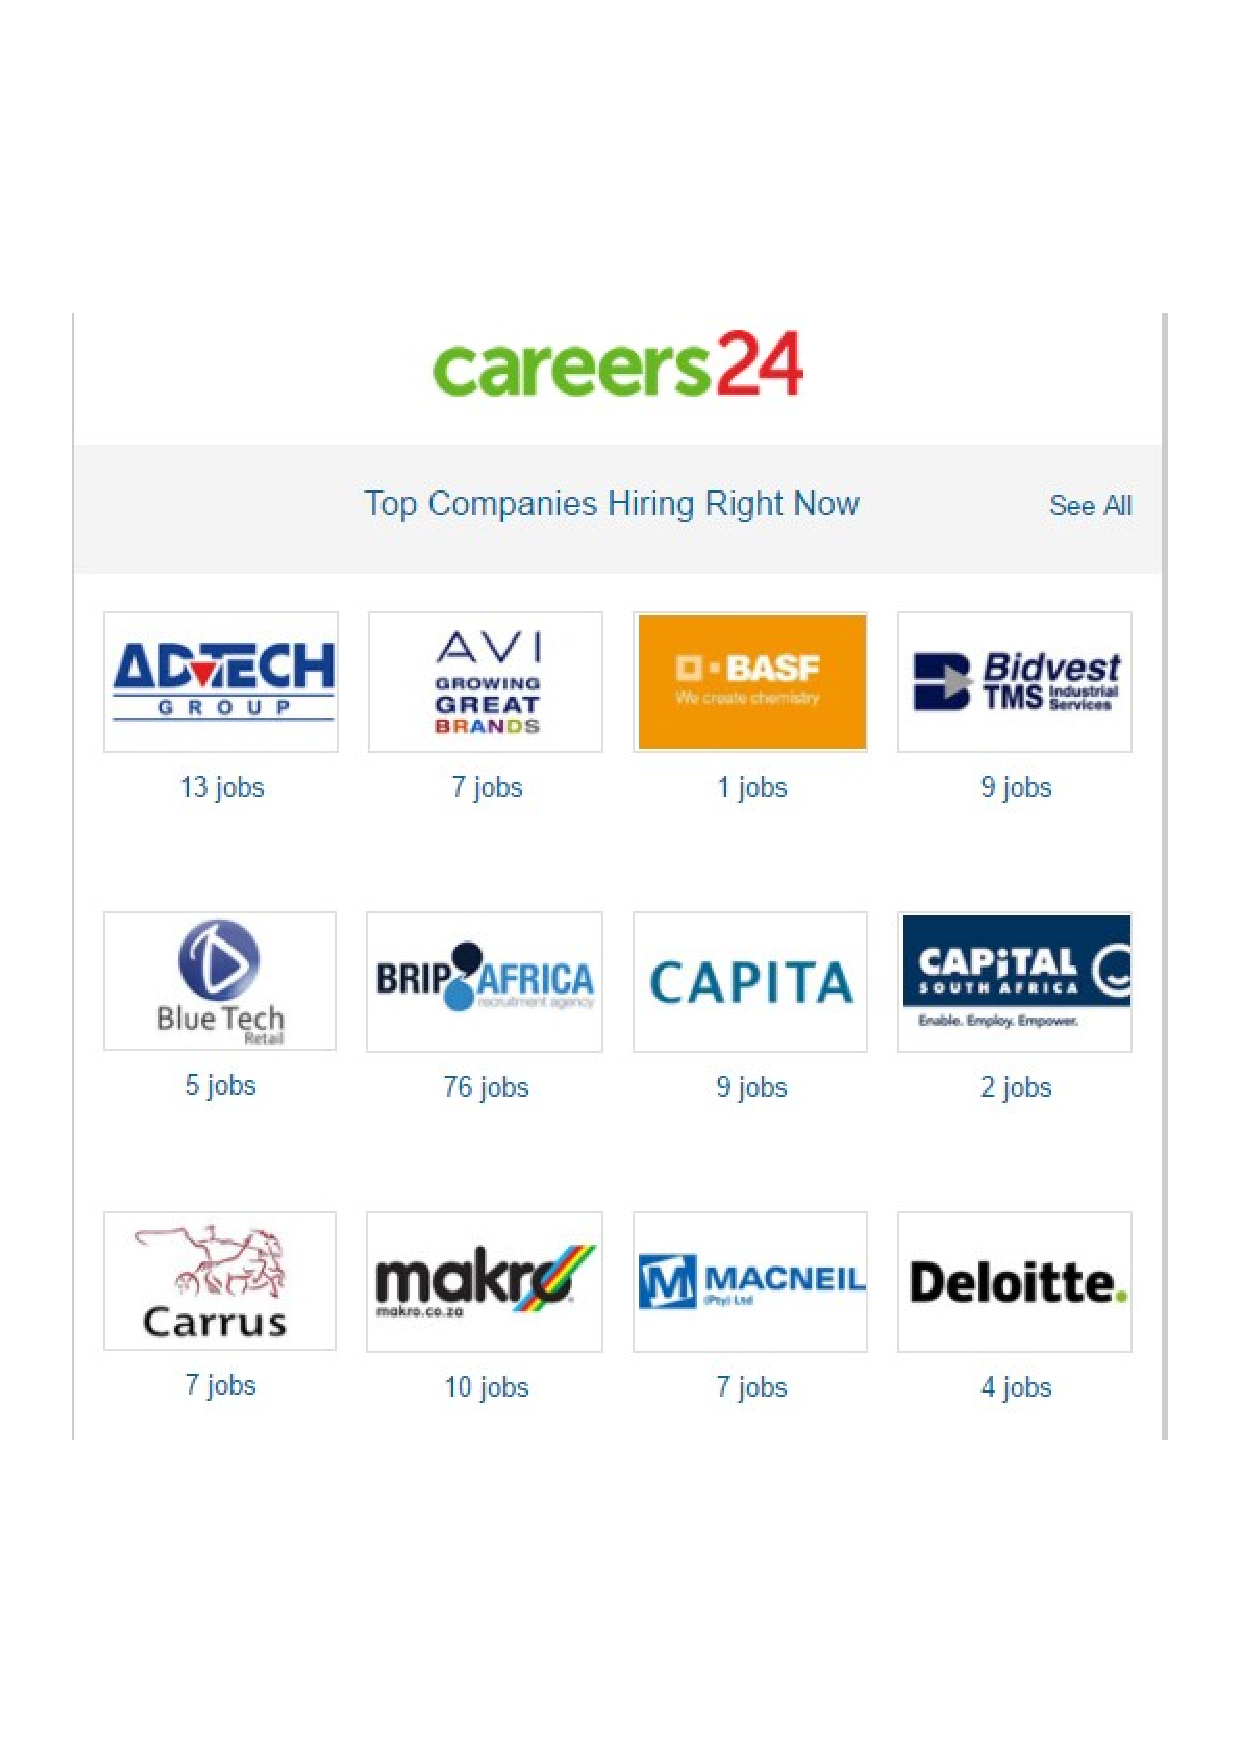
\includegraphics[width=0.75\linewidth]{dissertation/figures/Figure 12: Careers24 Jobs using Multimedia.pdf}
\caption{Careers24 Jobs using Multimedia}
\label{fig:careers24_multimedia}
\end{figure}

\FloatBarrier

%------------------------------------------------
\section{Language Learning}

The various ideas suggested in Table~\ref{tab:ict_enablers_part1} and Table~\ref{tab:ict_enablers_part2} can be developed to assist job seekers. Job seekers can benefit from a language learning application that teaches them the terminology for specific jobs in the language preferred by employers, in the South African context this could be English, Afrikaans or any of the 12 official languages.

%------------------------------------------------
\section{Co-design and ICTD Approach}

ICTD research should be embarked in a bottom-up manner where problems and recommended solutions are designed together by or with the community concerned to ensure researchers are well sensitized about the on-ground community situations and subsequently develop community embedded initiatives. Both the understanding of a problem as well as its solution should be Co-designed as the basis for emancipatory, well adopted, and sustainable development. Contrary to the approach in which several job-finding platforms have been developed from an employer-driven perspective, we Co-designed the development of our job finding platform making it job seeker-driven or more generally, driven by the affected. We found that when Co-design engages different sets of users for each cycle, there is a limited chance for users to become familiar with Co-design methods or tools and limited opportunity for the users to learn in their own way, however, there is a greater chance to get inputs from multiple users.

Although non-continuity meant we could not have each person’s views throughout the full research, employing different people to participate made for a rich final artefact with what works and what does not work for the Cape Town communities. We found that uncovering an issue such as unemployment was more openly discussed in a workshop with over 30 participants than a workshop of under ten people. We also found that participants could give divergent views when they were met on a one on one bases.

%------------------------------------------------
\section{Summary of Key Challenges}

Financial poverty, language non-proficiency, digital illiteracy, and skills poverty are the main issues faced in finding employment. The artefact designed in this study addresses language non-proficiency, digital illiteracy, and skills poverty to some extent, as discussed in this dissertation; however, there remains significant potential for ICT to be leveraged to alleviate all four areas.
